\documentclass{article}

\usepackage{pdfpages}

\usepackage[hidelinks]{hyperref}

\usepackage{array}
\usepackage{tabularx}

\usepackage{comment}

\usepackage{tcolorbox}

\usepackage{graphicx}
\usepackage{subcaption}

\usepackage{amsmath}

\usepackage{float}

\usepackage[export]{adjustbox}

\usepackage[margin=1.25in]{geometry}

\newtcbox{\inlinecode}{on line, boxrule=0pt, boxsep=0pt, top=2pt, left=2pt, bottom=2pt, right=2pt, colback=gray!15, colframe=white, fontupper={\ttfamily \footnotesize}}

\begin{document}
\pagenumbering{gobble}

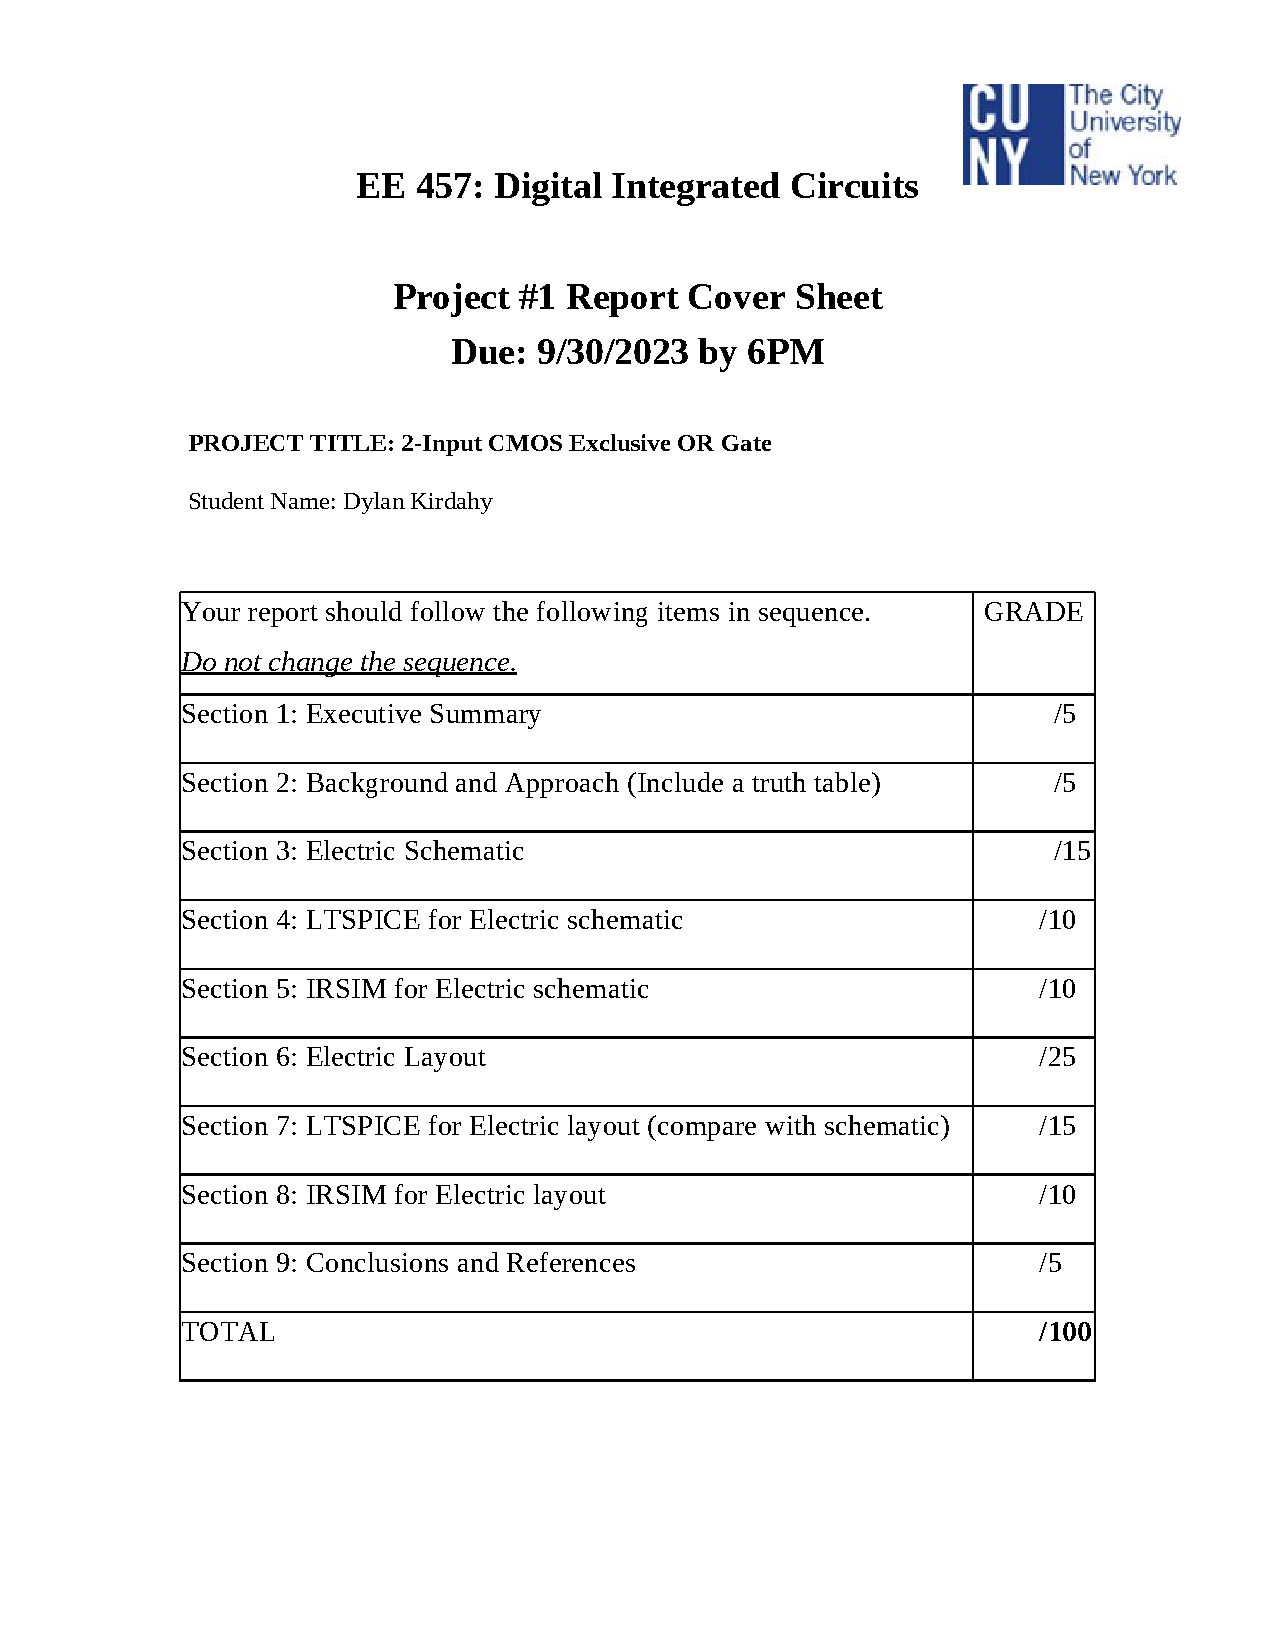
\includepdf[pages=-,scale=1,pagecommand={}]{project-1-cover-sheet.pdf}

\tableofcontents

\newpage
\pagenumbering{arabic}

\section{Introduction}

\paragraph{}
fjdsklfjdsklfjsklfsdj









\begin{comment}
%How to do inline code:
\paragraph{}
There is some inline code, \inlinecode{movff STATUS, STATUS\_TEMP}, in this sentence.

This formula $f(x) = x^2$ is an example of inline math.

\end{comment}


\begin{comment}
%How to do equations:

\begin{equation*}
P_{1f_m}=\int^\infty_{-\infty}G_{1f_m}(f)df=0.01\int^\infty_{-\infty}[\delta(f-2700)+\delta(f-2300)]df=0.01*(1+1)=0.02W
\end{equation*}


\end{comment}


\begin{comment}

%Here is a single figure
\begin{figure}[H]
  \centering
  \includegraphics[width=0.9\linewidth, frame]{screenshots/01.png}
  \caption{The system for this lab.}
  \label{fig:01}
\end{figure}

\end{comment}

\begin{comment}

%Here is a double figure
\begin{figure}[H]
  \centering
  \begin{subfigure}[b]{0.45\linewidth}
    \includegraphics[width=\linewidth, frame]{screenshots/02.png}
    \caption{The xyz block.}
  \end{subfigure}
  \begin{subfigure}[b]{0.45\linewidth}
    \includegraphics[width=\linewidth, frame]{screenshots/03.png}
    \caption{The abc block.}
  \end{subfigure}
  \caption{The two figures in this double figure.}
  \label{fig:02}
\end{figure}

\end{comment}


\end{document}
